%! TeX root = cheatsheet.tex

\documentclass[11pt,landscape,a4paper]{article}
\usepackage[utf8]{inputenc}
\usepackage[ngerman]{babel}
\usepackage{PTSansNarrow} 
\renewcommand*\familydefault{\sfdefault} %% Only if the base font of the document is to be sans serif
\usepackage[T1]{fontenc}
\usepackage[dvipsnames]{xcolor}
\usepackage{colortbl}
\usepackage{multicol}
\usepackage{multirow}
\usepackage{float}
\usepackage[top=0mm,bottom=1mm,left=0mm,right=1mm]{geometry}
\usepackage{microtype}
\usepackage{enumitem}
\usepackage{booktabs}
\usepackage{tikz}
\usetikzlibrary{arrows.meta,graphs,shapes.misc}
\usepackage{amssymb}
\usepackage{amsmath}
\usepackage{pifont}
\usepackage{listings}
\usepackage{xcolor}
\usepackage{mathtools}
\usepackage{graphicx}
\graphicspath{{src/}}

\newcommand{\cmark}{\ding{51}}%
\newcommand{\xmark}{\ding{55}}%

\lstdefinestyle{pseudo}{%
    backgroundcolor=\color{white},
    basicstyle=\ttfamily,
    numbers=left,
    numberstyle=\tiny\color{gray},
    keywordstyle=\color{blue},
    commentstyle=\color{gray},
    stringstyle=\color{orange},
    frame=single,
    breaklines=true,
    tabsize=4,
    morekeywords={Function,Return,If,Else,While,Begin,End}
}

\setlength{\jot}{0pt}
\appto{\footnotesize}{%
	\setlength{\abovedisplayskip}{0pt}
	\setlength{\belowdisplayskip}{0pt}
	\setlength{\abovedisplayshortskip}{0pt}
	\setlength{\belowdisplayshortskip}{0pt}
}

\newenvironment{Figure}
  {\par\medskip\noindent\minipage{\linewidth}}
  {\endminipage\par\medskip}

\pagestyle{empty}
\renewcommand{\baselinestretch}{0.9}

\makeatletter
\renewcommand{\section}{\@startsection{section}{1}{0mm}%
                                {.2ex}%
                                {.2ex}%x
								{\sffamily\small\bfseries}}
\renewcommand{\subsection}{\@startsection{subsection}{1}{0mm}%
                                {.2ex}%
                                {.2ex}%x
								{\sffamily\bfseries}}
\renewcommand{\paragraph}{\@startsection{paragraph}{1}{0mm}%
                                {.2ex}%
                                {.2ex}%x
								{\sffamily\bfseries}*}
\makeatother

\setlist[itemize]{noitemsep,nolistsep,leftmargin=*}
\setlist[enumerate]{noitemsep,nolistsep,leftmargin=*}
\setlength{\parindent}{0pt}
\setlength{\topsep}{0pt}
\setlength\multicolsep{0pt}

\definecolor{forestgreen}{rgb}{0.0, 0.27, 0.13}


\begin{document}
\footnotesize
\begin{multicols*}{4}
  \setcounter{section}{-1}
  \section{Compiled, Typed Languages}
\verb|java| $\xRightarrow{\text{compiled}}$ \verb|bytecode|
$\xRightarrow[\text{interpreted}]{\text{compiled}}$ \verb|machine code|\\
\textbf{Why Compile?} Able to debug while program is still
being developed\\
\textbf{Why not?} Source code is analysed
without running, cannot always ensure correctness $\Rightarrow$ Conservative /
Permissive Checking\\
\textcolor{OliveGreen}{eg.}
$CTT(\verb|c|)=\verb|Shape|$, $RTT(\verb|c|)=\verb|Circle|$
\begin{verbatim}
Shape c = new Circle();
c.getRadius();
\end{verbatim}
\paragraph{Type Conversions}
Suppose $\verb|S|<:\verb|T|$.
Then implicit type conversion from \verb|S| to \verb|T| (narrowing) is allowed.
Type conversion from \verb|T| to \verb|S| (widening) requires type casting.

	\section{Abstraction}
The \emph{separation of concerns} between implementor and client.
\begin{itemize}
  \item Compartmentalise computation \& effects
  \item Hide implementation of tasks $\Rightarrow$ able to change
  \item Reduce code complexity through code reuse
\end{itemize}
\begin{center}
  \vspace{-1mm}
  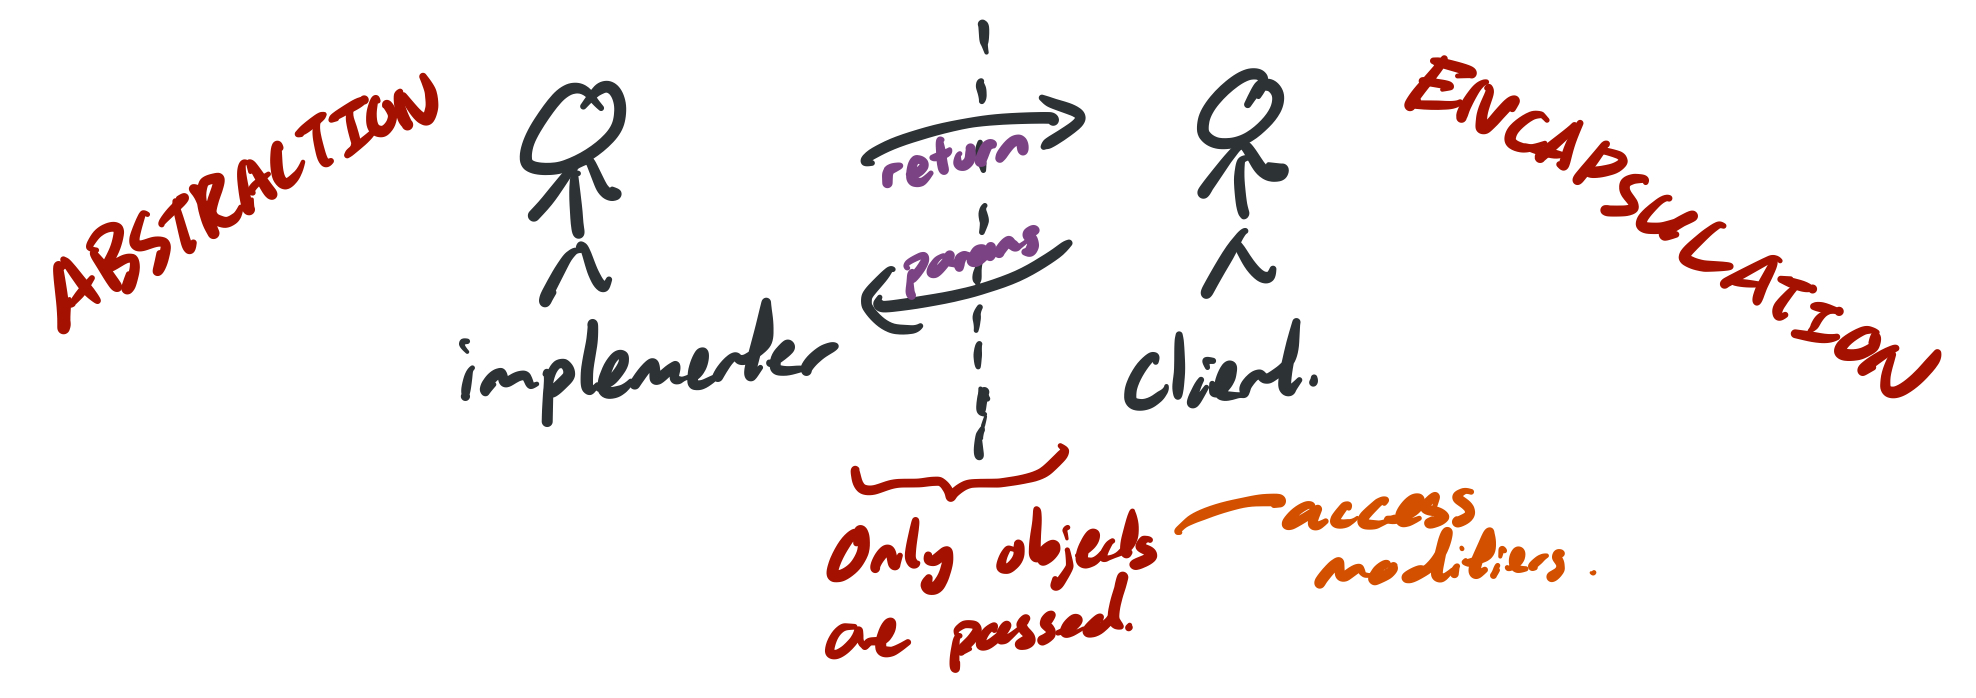
\includegraphics[width=0.8\linewidth]{abstraction}
\end{center}
\vspace{-5mm}
% \paragraph{Variables}
% An abstraction over data: giving a name to the piece of data.\\
% Type systems: \textcolor{OliveGreen}{Dynamic} vs.
% \textcolor{Bittersweet}{Static} (Weak $\leftrightarrow$ Strong)
% \paragraph{Functions}
% An abstraction over a set of instructions
% \paragraph{Composite Data Types}
% An abstraction over a group of primitive types
% \paragraph{Class an Object}
% An abstraction over a composite data type and associated functions

  \section{Encapsulation}
Abstraction over types/functions, exposing \emph{ONLY} a certain interface
\begin{itemize}
  \item Ability to create complex data types
  \item Creates an abstraction barrier
\end{itemize}
\paragraph{Composition}
Models a \emph{HAS-A} relationship. Further abstraction and encapsulation.\\
\textcolor{Bittersweet}{Dangers of Aliasing}: Sharing references between objects
\paragraph{Information Hiding}
To enforce the abstraction barrier using access modifiers, to avoid direct
access to info and data

\begin{tabular}{c c c c c c}
  & \multirow{2}{*}{Same class} & \multicolumn{2}{c}{Same Package} & \multicolumn{2}{c}{Different Package}\\
  & & Sub & Non-Sub & Sub & Non-Sub\\
  private &\textcolor{OliveGreen}{\cmark}&\textcolor{Bittersweet}{\xmark}&\textcolor{Bittersweet}{\xmark}&\textcolor{Bittersweet}{\xmark}&\textcolor{Bittersweet}{\xmark}\\
  default &\textcolor{OliveGreen}{\cmark}&\textcolor{OliveGreen}{\cmark}&\textcolor{OliveGreen}{\cmark}&\textcolor{Bittersweet}{\xmark}&\textcolor{Bittersweet}{\xmark}\\
  protected &\textcolor{OliveGreen}{\cmark}&\textcolor{OliveGreen}{\cmark}&\textcolor{OliveGreen}{\cmark}&\textcolor{OliveGreen}{\cmark}&\textcolor{Bittersweet}{\xmark}\\
  public &\textcolor{OliveGreen}{\cmark}&\textcolor{OliveGreen}{\cmark}&\textcolor{OliveGreen}{\cmark}&\textcolor{OliveGreen}{\cmark}&\textcolor{OliveGreen}{\cmark}
\end{tabular}

\paragraph{Tell, Don't Ask}
\textcolor{OliveGreen}{Telling the object what to do}, instead of
\textcolor{Bittersweet}{Asking for state} + Performing task on behalf. 
\begin{itemize}
  \item Prevent leakage of class implementation details
  \item Keep encapsulation intact
  \item Reduce coupling between client and class
\end{itemize}
Tasks performed only on fields should be implemented in the class


  \section{Inheritance}
\verb|Subclass| <: \verb|Superclass|\\
Models the \emph{IS-A} relationship. To extend certain properties of classes.
\textcolor{Bittersweet}{Technically breaks the abstraction barrier}\\
\verb|final| Keyword in declarations to prevent class inheritance, method
overriding and field re-assignment
\paragraph{Method Overriding \& Overloading}
\textcolor{Blue}{Method Signature}: Number, type, order of params., and name\\
\textcolor{Blue}{Method Descriptor}: Method Signature + Return type\\
\verb|@Override|: When subclass defines an \emph{instance} method with the same
method signature, a return sub-type, and throws sub-type checked exception, or
doesn't throw an exception\\
Overloading: When class defines two or more methods with the same name but
different method signatures.
\paragraph{Liskov Substitution Principle}
Let $\phi(x)$ be a property provable $\forall x$ of type \verb|T|. Then
$\phi(y)$ should be true $\forall y$ of type \verb|S| where
$\verb|S|<:\verb|T|$, ie.\\
$\Rightarrow$ Subclass is substitutable, and pass all test cases of superclass
$\Rightarrow$ Ensures inheritance with method overriding is safe\\
\textcolor{Bittersweet}{Needs to be enforced by programmer, not compiler}
\paragraph{Inheriting}
Classes can extend $\le1$ superclasses, implement $\ge0$ interfaces.\\
Interfaces can extend $\ge0$ interfaces.
\begin{itemize}
  \item \textcolor{Blue}{Abstract Class}
    \begin{itemize}
      \item Allow general \& extensible code writing for other classes
      \item To demonstrate \emph{IS-A} relationships, without specific implementation
      \item May have no abstract method
      \item Cannot be instantiated
    \end{itemize}
  \item \textcolor{Blue}{Interface}
    \begin{itemize}
      \item Modelling behaviour across class hierachies
      \item Methods are \verb|public abstract|
      \item Fields are \verb|public static final|
    \end{itemize}
\end{itemize}
\textcolor{Bittersweet}{Note}: \emph{ANY} object can be casted to \emph{ANY} interface

  \section{Polymorphism}
Difference in code behaviour without changing existing code. Allows succinct,
future-proof code.
\paragraph{Dynamic Binding}
Determining which method to be invoked from RTT of object.
\verb|x.invokedMethod(params...)|
\begin{enumerate}
  \item During compile time
    \begin{enumerate}
      \item Determine method descriptor of invoked method with \verb|CTT(x)|
      \item Search \emph{ALL} methods in \verb|CTT(x)| that can be invoked
    \item Choose the \emph{most specific} method.\ \textcolor{Bittersweet}{If none exists, error.}
      \item Store method descriptor in the bytecode
    \end{enumerate}
  \item During run-time
    \begin{enumerate}
      \item Retrieve method descriptor from bytecode
      \item Search for first matching method:\\
        $\Rightarrow$ Starting from \verb|RTT(x)|, iterating to parent class
    \end{enumerate}
\end{enumerate}
\textcolor{Blue}{Most Specific Method}: If arguments to \verb|M| can be passed
into \verb|N| without compilation error, \verb|M| is more specific than
\verb|N|

\textcolor{Bittersweet}{Class Methods}: No Dynamic Binding. Step 1 taken and
CTT's method is executed.

  \section{Heap and Stack}
The Heap stores dynamically allocated objects. Persists across method
invocations. Dealloc $\iff!\exists$ reference\\
The Stack (actual stack) stores variables, and call frames. $\varnothing$ for
uninitialised variables. Dealloc when method returns\\
\begin{center}
  \vspace{-4mm}
  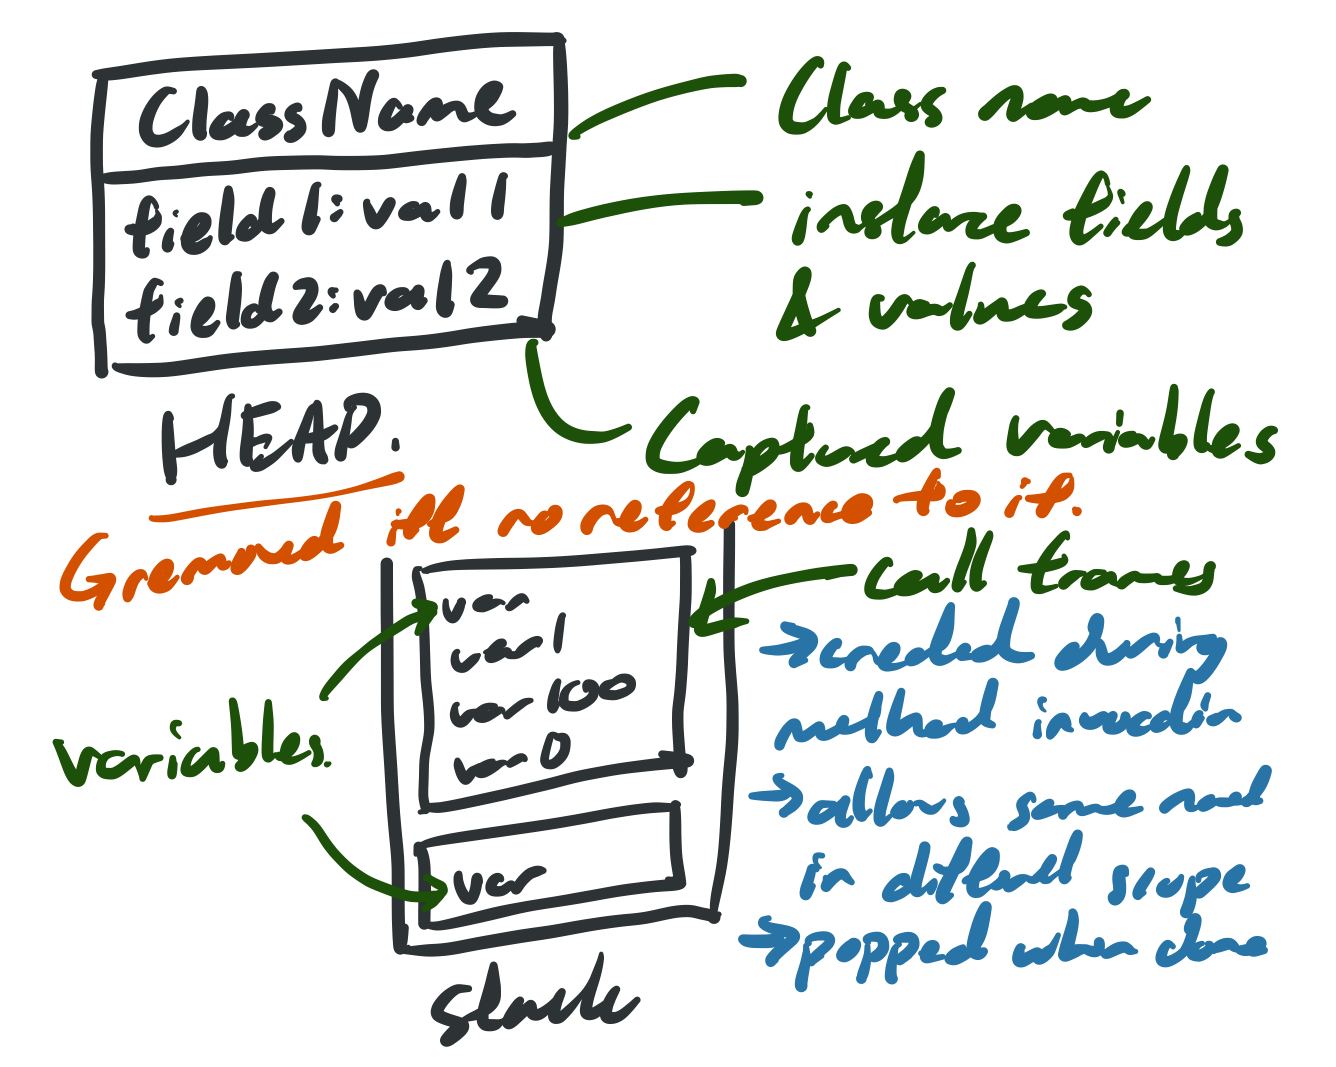
\includegraphics[width=0.5\linewidth]{heapandstack}
\end{center}
\vspace{-5mm}
\paragraph{Primitive Types}
\begin{center}
 $\verb|byte|<:\verb|short|<:\verb|int|<:\verb|long|<:\verb|float|<:\verb|double|$\\
 $\verb||\verb|char|<:\verb|                   |$
\end{center}
\textcolor{Bittersweet}{Note}: 
\begin{itemize}
  \item Uninitialised fields have default values, but not variables
  \item Methods call by value for primitives, call by reference for objects
\end{itemize}
\paragraph{Wrapper Classes}
Encapsulates the primitive types to write general code for all reference types.
Immutable $\Rightarrow$ Much more expensive than primitives.
\begin{verbatim}
Integer i = Integer.valueOf(4);
int j = i.intValue();
\end{verbatim}
Type conversion between primitive and wrapper done by
\textcolor{Blue}{auto-boxing} and \textcolor{Blue}{unboxing}
\textcolor{Bittersweet}{ONLY} with the equivalent wrappers.

  \section{Exceptions}
\begin{verbatim}
try { // do something }
catch (Exception e) { // handle exception }
finally { // clean up
   // no matter exception occurred or not 
}
\end{verbatim}
\begin{center}
  \vspace{-5mm}
  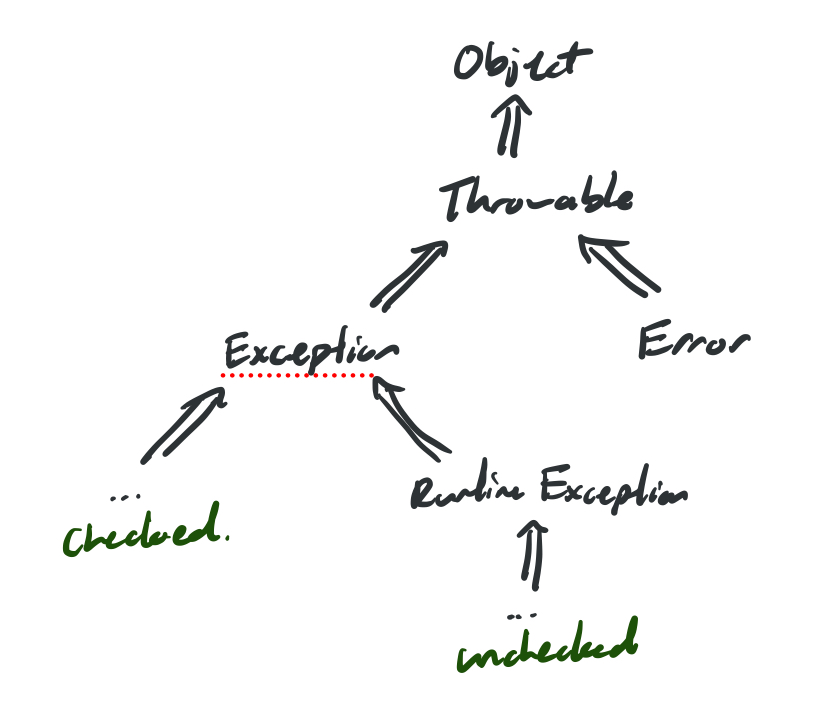
\includegraphics[width=0.5\linewidth]{exception}
  \vspace{-4mm}
\end{center}
\textcolor{Blue}{Checked exceptions} might still happen with perfect code,
programmer has no control.  Must be handled to compile.\\
\textcolor{Blue}{Unchecked exceptions} are caused by programmer errors that cause
Runtime Exceptions.
\paragraph{Catch}
\begin{verbatim}
} catch (ExceptionX e) { 
   ...
} catch (ExceptionY e) {
\end{verbatim}
Exceptions are checked in order. If $\verb|ExceptionY|<:\verb|ExceptionX|$, the
second catch will never run $\Rightarrow$ \textcolor{Bittersweet}{Exception!}
\paragraph{Design principles}
\begin{enumerate}
  \item Catch exceptions to clean up, even if just ``passing the buck''
  \item Do NOT catch all (Exception e)
  \item Do not overreact (Exiting the program)
  \item Do not break abstraction (Leaking abstraction throwing \verb|FileNotFound| etc.)
  \item Do not use as flow control mechanism
\end{enumerate}

  \section{Complex Types}
\paragraph{Variance of Types}
Let $C(S)$ be some complex type based on $S$.\\
$C$ is Covariant $\iff (S<:T \rightarrow C(S)<:C(T))$\\
$C$ is Contravariant $\iff (S<:T \rightarrow C(T)<:C(S))$\\
$C$ is Invariant $\iff C$ is not covariant $\wedge\ C$ is not contravariant
\paragraph{Arrays}
Covariant for reference types \textcolor{Bittersweet}{ONLY}.\\
Technically violates the LSP\@. Unable to put \verb|Object| in \verb|Integer[]|,
even though $\verb|Integer[]|<:\verb|Object[]|$

  \section{Generics}
A generic type takes other types as type parameters.\\
\textcolor{Blue}{Generic Class} Pair<S,T> with \textcolor{Blue}{Type
Parameters} \verb|S, T| \textcolor{Bittersweet}{$\leftarrow$ SCOPED}\\
\textcolor{Blue}{Type Arguments} \verb|String, Integer| are passed in, to
create\\
\textcolor{Blue}{Parametrised Type} \verb|Pair<String, Integer>|
\textcolor{Blue}{Generic Methods} are methods that are parameterised with type
parameters
\paragraph{Type Erasure}
Implementation of Generics in Java: \textcolor{ForestGreen}{Code Sharing}.
After type checking, type parameters and arguments are erased.\\
\textcolor{Gray}{Alternative: Code Specialisation–Code for every
instantiated type.}\\
We denote $|T|$ for the erasure of type $T$.
\begin{itemize}
  \item The erasure of a parameterized type \verb$G<T1,\ldots,Tn>$ is \verb$|G|$.
  \item The erasure of a nested type \verb$T.C$ is \verb,|T|.C,.
  \item The erasure of an array type \verb.T[]. is \verb+|T|[]+.
  \item The erasure of a type variable is the erasure of its leftmost bound.
  \item The erasure of every other type is the type itself.
\end{itemize}
\emph{Bridging Methods} are generated when the class extends a parameterised
type, to match the type erased signature of the parent class's method.
\begin{verbatim}
public void foo(Object arg) {
   foo((Param-edType) arg);
} // Bridging Method
public void foo(Param-edType arg) { ... }
\end{verbatim}
\paragraph{Reifiable Types}
Where type information is fully available at runtime–none erased during
compilation. A
type is \emph{reifiable} $\iff$ any of the following:
\begin{itemize}
  \item It refers to a non-generic class or interface type declaration.
  \item It is a parameterized type in which all type arguments are unbounded wildcards.
  \item It is a raw type: Generic Class or Interface without type arguments.
    \textcolor{Bittersweet}{DO NOT USE\@. No type checking at all.}
  \item It is a primitive type.
  \item It is an array type whose element type is reifiable.
  \item It is a nested type, for each type \verb$T$ separated by a \verb$.$, \verb$T$ is reifiable.
\end{itemize}
\textcolor{ForestGreen}{Arrays' Reifiability} allows covariance: When a
variable of the wrong type is put in the array, it throws a
\verb$RuntimeException$. \\
Type refiability prevents \textcolor{Bittersweet}{\textbf{Heap
Pollution}}–where a variable of a parameterised type refers to an object not of
that parameterised type.\\
\textcolor{Blue}{Resolved by}: Invariance of Generics, and Checking type safety during compile time\\
\textcolor{Blue}{To create Generic Type Arrays}: Ensure no heap pollution $\Rightarrow$
\verb$@SuppressWarnings("unchecked")$ on array \emph{declaration}
\paragraph{Bounding Type Parameters}
Constraining valid type arguments, to allow assert certain properties or method
usages: \verb|T extends U, R super S|\\
\textcolor{Blue}{Wildcards} To write general code despite generic invariance:
Enforce subtyping relationships on type arguments.\\
\begin{center}\vspace{-3mm}\textcolor{Bittersweet}{\textbf{Producer Extends,
Consumer Extends}}\end{center}
Whether the variable ``\emph{produces}''–returns variables of type \verb|T|–or
``\emph{consumes}''–accepts variables of type \verb|T|\\
\textcolor{ForestGreen}{Unbounded Wildcards} \verb$T<?>$ is the maximum element
of the partial order $<\colon$. BUT \verb$CTT(T<?>.produce())=Object$, \verb$T<?>.consume(null)$ ONLY
\paragraph{Type Inference}
When type witness is unspecified: Calling a generic method, or using the diamond operator.
\begin{enumerate}
  \item A bound set is generated from a list of type
    parameter declarations $P_1,\ldots,P_p$ and associated inference variables
    $\alpha_1,\ldots,\alpha_p$ to be determined. For each $l\in\{1..p\}$:
    \begin{itemize}
      \item If $P_l$ has no bound, $\alpha<\colon Object$ is added.
      \item Otherwise, for each $T$ delimited by $\&$ in the bound, $\alpha_1<\colon T$ is added.
      \item If no proper upper bound for $\alpha_l$ is added, $\alpha_l<\colon Object$ is added.
    \end{itemize}
  \item Reduction: Simplifying a set of constraint formulas into a bound set.
    Constraint formulas are given by:
    \begin{itemize}
      \item Type of return variable: Target Typing
      \item Type of Method Arguments
    \end{itemize}
  \item Incorporation: To infer new bounds based on assertions of original bounds.
  \item Resolution: For a bound set that does not contain the bound $false$, a
    subset of the inference variables may be resolved.
    \begin{itemize}
      \item If $\alpha_i$ has one or more proper lower bounds $L_1,\ldots,L_k$,
        $T_i=\operatorname{lub}(L_1,\ldots,L_k)$
      \item Otherwise, if $\alpha_i$ has one or more proper upper bounds
        $U_1,\ldots,U_k$, $T_i=\operatorname{glb}(U_1,\ldots,U_k)$
    \end{itemize}
\end{enumerate}
\begin{center}
  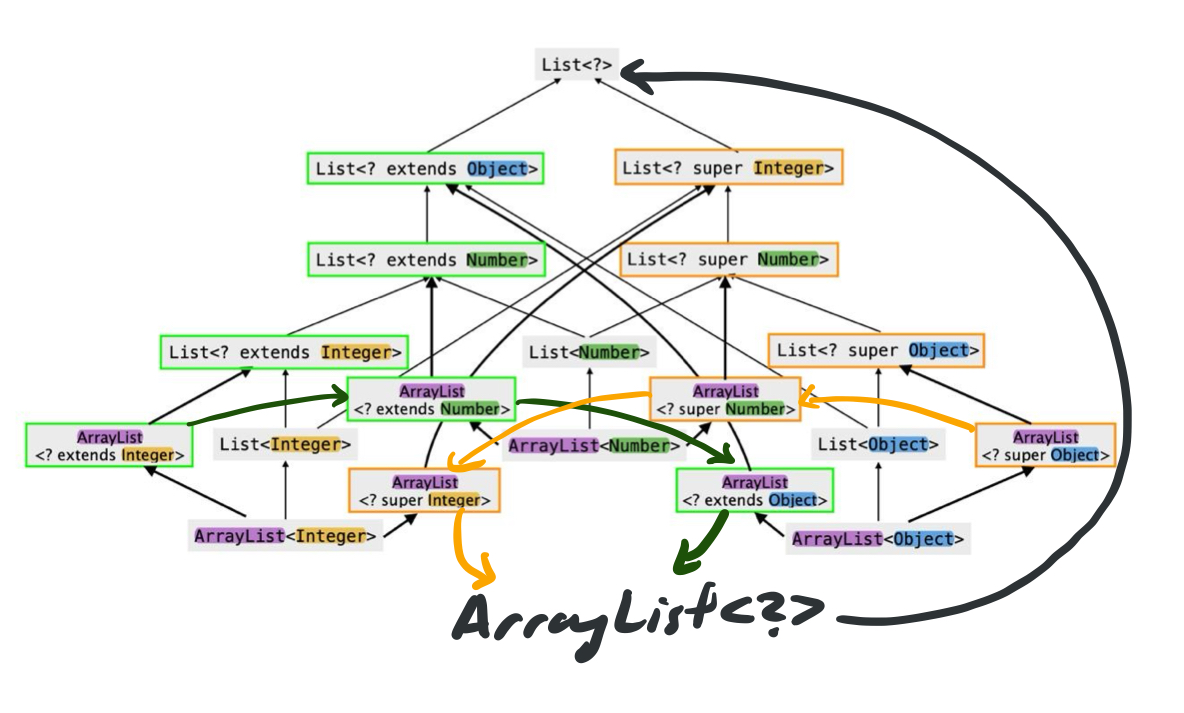
\includegraphics[width=\linewidth]{generictypes}
\end{center}

  \section{Functional Programming}
Avoiding change altogether
\begin{itemize}
  \item Ease of reasoning and understanding
  \item Enable safe sharing of objects: \textcolor{ForestGreen}{Cached single copy of origin}
  \item Enable safe sharing of internals: \textcolor{ForestGreen}{Return new
    object with same cached array with different start/end indices etc.}
  \item Enable safe concurrent execution \textcolor{Bittersweet}{$\iff$ no
    mutation within abstraction barrier}
\end{itemize}
\subsection{Referential Transparency}
Suppose \verb$s.get(0)$ returns \verb$k$.\\
\textcolor{Blue}{Deterministic and Immutable}: We are then able to replace all invocations of \verb$s.get(0)$
with \verb$k$, and \\
\textcolor{Blue}{No Side Effects}: usages of \verb$T t = s.get(0)$ with \verb$s.get(0)$.
\paragraph{Immutability}
Instances with no visible changes outside abstraction barrier
$\Rightarrow$ Every call of the instance's method behaves the same way
throughout the lifetime of the instance. How:
\begin{enumerate}
  \item Prevent Inheritance: \textcolor{Bittersweet}{IMPT\@! Ensure no change in behaviour}
  \item Prevent field reassigning: Ensure no mutation of fields
  \item Prevent field mutation: Fields have to be immutable
\end{enumerate}
\paragraph{No Side Effects}
\begin{multicols*}{2}
\begin{itemize}
  \item Printing to screen
  \item Writing to files
  \item Throwing Exceptions
\end{itemize}
\begin{itemize}
  \item Changing other variables
  \item Modifying arguments
\end{itemize}
\end{multicols*}
\textcolor{ForestGreen}{void functions, and division operations} are not pure.
\textcolor{Bittersweet}{Overflow} is not an error.

  \section{Nested Classes}
Defining a class within another class/method, to group logically relevant
classes within the same encapsulation.\\
\textcolor{Bittersweet}{NOTE:\@ Container class CAN access private fields of
nested class!}
\begin{verbatim}
public/[default] class OuterClass {
   static class StaticNestedClass { ... }
   class InnerClass { ... }
}
\end{verbatim}
\paragraph{Access Modifiers}
Nested classes can be \verb$private$, \verb$protected$, \verb$[default]$,
\verb$public$. Private nested classes' instances can still be returned and
exist outside of the class, but their methods and fields cannot be used, even
if they are \verb$public$.\\
Should only be exposed $\iff$ no implementation details leaked, and is an essential part of
interface of outer class.
\subsection{Static Nested Class}
Associated with the containing \emph{class}. Can only access \textcolor{Blue}{static
fields and methods} of containing class.
\begin{verbatim}
Outer.Inner iObj = new Outer.Inner();
\end{verbatim}
\subsection{Inner Class}
Associated with the containing \emph{instance}. Can access \textcolor{Blue}{all
fields and methods} of containing class.
\begin{verbatim}
Outer oObj = new Outer();
Outer.Inner iObj = oObj.new Inner();
\end{verbatim}
\paragraph{Local Class}
Class defined within a function, scoped within the method. Can access
\textcolor{Blue}{fields and methods} of containing class, and
\textcolor{Blue}{local variables} of enclosing method. A local class in a
static method can only access static members of the containing class.
\paragraph{Anonymous Class}
Declaration AND instantiation of a local class in a single statement.
\begin{center}
  \verb$new SuperClass(args) { body }$
\end{center}
Fields, extra methods, instance initialisers and local classes are allowed in
\verb$body$, like a normal class \textcolor{Bittersweet}{without constructors}.
\subsection{Variable Capture}
Creating a copy of local variables inside the local class.\ \emph{Language
design decision} to only allow variables that are \verb$final$
\textcolor{Bittersweet}{or ``effectively final''}. Mutation not by
reassignment is still allowed.
\paragraph{Shadowing}
When the inner class declares a variable with the same name as one of the
enclosing class, it shadows the variable.\\
\verb$this.x$ refers to the inner class' member, while \verb$Outer.this.x$
refers to the outer class' member.
\paragraph{Stack and Heap}
On the stack and heap, a new instance of this class will include a copy of the
variables required in the inner class, \verb$Outer.this$, and the inner class'
variables.
\subsection{Lambda Expression}
\begin{center}
  \verb$@FunctionalInterface$
\end{center}
for interfaces with exactly \textbf{one} abstract method. Able to use lambda
expressions as syntactic sugar to simplify \emph{usage of functions as
first-class citizens}.\\
Similar to anonymous classes without introducing a new level of scoping.
Declarations, and variable references are \emph{interpreted just as they are}
in the enclosing environment. No shadowing issues \verb$:)$
\textcolor{Bittersweet}{Not allowed to redeclare variables, even as a parameter.}
\paragraph{Curried Functions}
\begin{center}
  $(X,Y)\rightarrow Z\equiv X\rightarrow Y\rightarrow Z$
\end{center}
Translating a $n$-ary function to a sequence of $n$ unary functions–a
higher-order function. Each lambda expression is a \textcolor{Blue}{closure},
\emph{storing data from the environment} where it is defined.
\paragraph{Method Referencing}
Referencing an existing method rather than specifying a new lambda. Can be used for:
\begin{itemize}
  \item Static method \verb$A::foo$ $\Rightarrow$ \verb$(args) -> A.foo(args)$
  \item Instance method\\
    \verb$aObj::foo$ $\Rightarrow$ \verb$args -> aObj.foo(args)$\\
    \verb$A::foo$$\Rightarrow$\verb$(args[1..])->args[0].foo(args[1..])$
  \item Constructors \verb$A::new$ $\Rightarrow$ \verb$args -> new A(args)$
\end{itemize}
During compilation, type inference is used to match the given reference to a
matching method.\ \textcolor{Bittersweet}{Compilation Error} if multiple matches
or ambiguity.

  \section{Monads}
Equipped with two functions \verb|of| and \verb|flatMap| satisfying the laws:
\begin{enumerate}
  \item Left Identity Law\\
    $\verb|Monad.of|(x)\verb|.flatMap|(x\rightarrow f(x))\equiv f(x)$
  \item Right Identity Law\\
    $\verb|m.flatMap|(x\rightarrow\verb|Monad.of|(x))\equiv\verb|m|$
  \item Associative Law\\
    $\verb|m.flatMap|(x\rightarrow f(x))\verb|.flatMap|(y\rightarrow g(y))\equiv\\
     \verb|m.flatMap|(x\rightarrow f(x)\verb|.flatMap|(y\rightarrow g(y)))$
\end{enumerate}
\paragraph{Functor}
\begin{center}
  $\verb|Monad|\Rightarrow\verb|Functor|\quad\verb|Functor|\nLeftarrow\verb|Monad|$
\end{center}
Sufficient for lambdas to be applied sequentially to a value.
\begin{enumerate}
  \item Identity Preservation\\
    $\verb|f.map|(x\rightarrow x)\equiv\verb|f|$
  \item Composition Preservation\\
    $\verb|f.map|(x\rightarrow f(x))\verb|.map|(x\rightarrow g(x))\equiv\\
    \verb|f.map|(x\rightarrow g(f(x)))$
\end{enumerate}

  \section{Concurrency and Parallelelisation}
\textcolor{Blue}{Parallelism}: multiple subtasks run at the same time, with a
processor that runs multiple instructions, or with multiple processors.\\
\textcolor{Blue}{Concurrency}: the ``illusion'' of parallelism.
\begin{center}
  $Parallel\Rightarrow Concurrent,Concurrent\nLeftarrow Parallel$
\end{center}
Parallelisation is \textcolor{Bittersweet}{non-deterministic}: no order of
which processes start and complete.
\paragraph{Parallelisability}
\begin{itemize}
  \item No Interference: No modification of the stream during execution of
    terminal operation. Throws
    \textcolor{Bittersweet}{ConcurrentModificationException}
  \item Stateless: The result does not depend on any state that might change
    during executiion of the stream \textcolor{ForestGreen}{Previous elements,
    Input}
  \item No Side-effects: No concurrent modification of non-thread safe objects
    that may result in incorrect behaviour
\end{itemize}
Operations that fulfil these conditions are known as \textcolor{Blue}{embarrassingly parallel}.
\begin{center}
  Parallelising $\neq$ Performance
\end{center}
Creating too many threads will \textcolor{Bittersweet}{outweigh benefits} of
parallelisation.
For \textbf{streams}, particularly for
\begin{verbatim}
stream.reduce(U i,
   BiFunc<U, ? super T, U> acc,
   BinOp<U> comb>)
\end{verbatim}
which accumulates each substream and combines the result, parallelisation
further requires:
\begin{itemize}
  \item $\verb|combiner.apply(i, x)|\equiv\verb|x|,\forall x$
  \item \verb|combiner| and \verb|accumulator| are associative.
  \item \verb|combiner| and \verb|accumulator| are compatible.\\
  $\verb|comb.apply(u, acc.apply(i, v))|\equiv\\\verb|acc.apply(u,v)|,\forall u,v$
\end{itemize}
Streams themselves may define encounter order:
\begin{multicols*}{2}
  \textcolor{ForestGreen}{\textbf{Ordered}}
  \begin{itemize}
    \item \verb$Stream::iterate$
    \item \verb$Stream::of$
    \item Ordered Collections
  \end{itemize}
  \textcolor{Bittersweet}{\textbf{Unordered}}
  \begin{itemize}
    \item \verb$Stream::generate$
    \item Unordered Collections
  \end{itemize}
\end{multicols*}
Operations that respect encounter order: \verb|distinct|, \verb|sorted|,
\verb$findFirst$, \verb$limit$, \verb$skip$ are expensive.
\verb|stream.unordered()| if original order is not important.
\paragraph{Threads}
In Java, threads divide computation into subtasks, to improve utilisation of
processor.
\begin{center}
  \verb$new Thread(RUNNABLE).start();$
\end{center}
The execution flow of each thread can be separately programmed with
\verb$Runnable.run()$. Program exits only after \emph{ALL} created threads run
to their completion.
\paragraph{CompletableFuture<T>}
\emph{A MONAD}. A \verb$CF$ is either completed or not complete.\\
To \textbf{Create a CF}:
\begin{itemize}
  \item \verb|CF<U> CF.completedFuture(U value)|
  \item \verb|CF<Void> runAsync(Runnable r)|
  \item \verb|CF<T> supplyAsync(Supplier<T> s)|
\end{itemize}
To \textbf{Chain CFs}:
\begin{itemize}
  \item \verb|CF<Void> thenAccept(Consumer<T> c)|
  \item \verb|CF<U> thenApply(Function<T, U> map)|
  \item \verb|CF<U> thenCompose(Function<T, CF<U>> map)|
  \item \begin{verbatim}
CF<U> thenCombine(CF<V> other,
                  BiFunc<T, V, U> fn)
    \end{verbatim}
  \item \verb|CF<Void> thenRun(Runnable r)|
\end{itemize}
To \textbf{get CF result}:
\begin{itemize}
  \item \verb|T get()| throws \textcolor{Bittersweet}{InterruptedException, ExecutionException}
  \item \verb|T join()| throws any \textcolor{Bittersweet}{Exception} that occurs
\end{itemize}
\textbf{Handling Exceptions}:
\begin{itemize}
  \item \verb|CF<T> exceptionally(Func<Throwable, T> f)|
  \item \verb|whenComplete(BiCons<T, Throwable> cons)|
  \item \verb|CF<R> handle(BiFunc<V, E, R> f)|
\end{itemize}
\begin{center}
  \vspace{-4mm}
  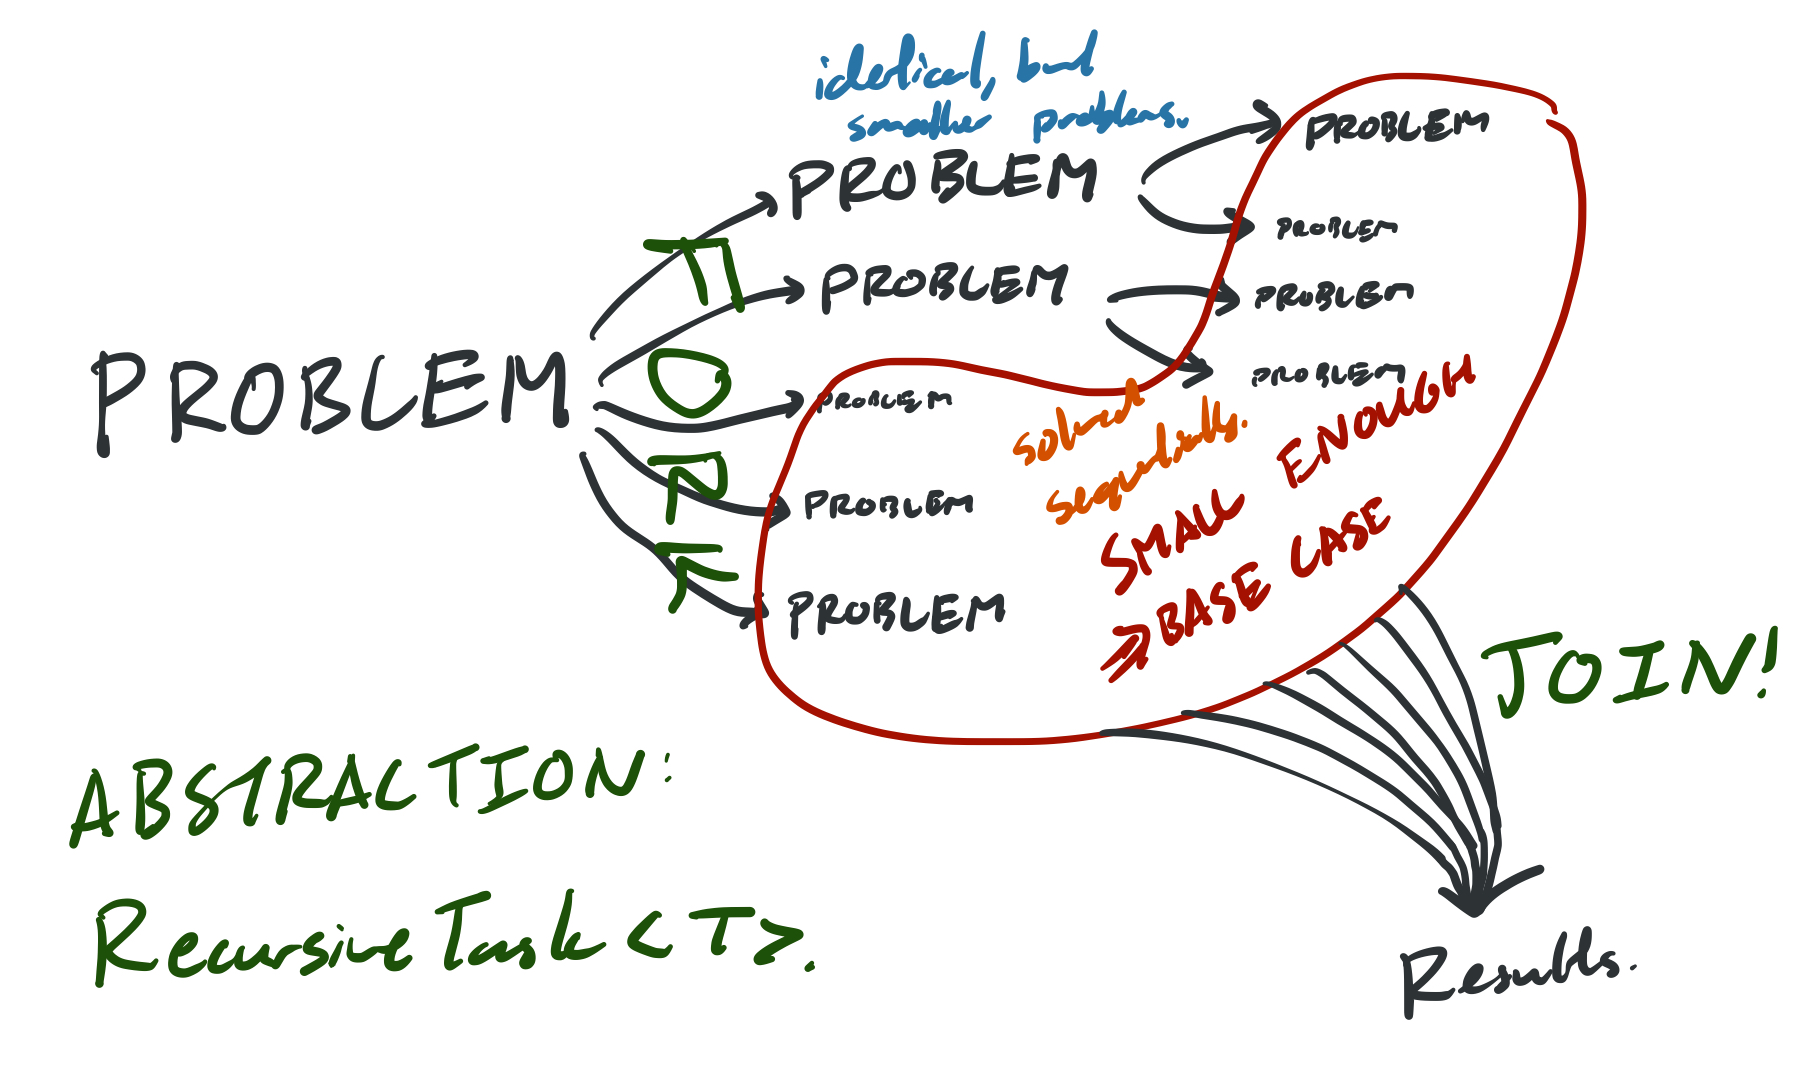
\includegraphics[width=\linewidth]{recursivetask}
  \vspace{-5mm}
\end{center}
\begin{enumerate}
  \item Idle Thread: Take head of own deque. If empty, take tail of another deque, and compute.
  \item \verb|fork()| called: Invoker adds itself to the head of current deque.
  \item \verb|join()| called: If complete, read result and join returns. If not
    stolen, compute on current thread. If stolen, do another task while waiting.
\end{enumerate}
Order of fork join: ``Palindrome'', with only ONE compute in the middle

\end{multicols*}
\end{document}
